\documentclass[crop, tikz]{standalone}
\usepackage{tikz}
\usetikzlibrary{arrows.meta, calc, positioning, shapes.misc}

\begin{document}
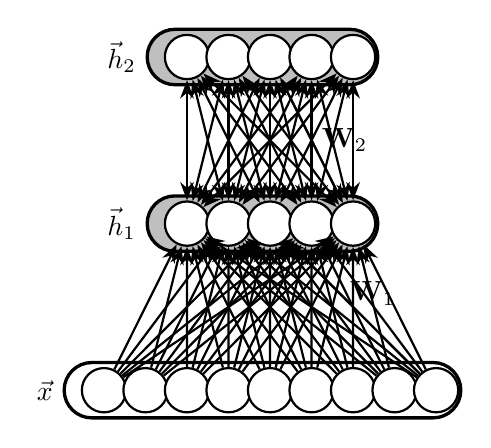
\begin{tikzpicture}[
  >=Stealth,
  pill/.style={draw, very thick, rounded rectangle, minimum height=2em},
  unit/.style={circle, draw, thick, minimum size=1.6em, fill=white},
]
  \node[pill, minimum width=15em] (x) {};
  \node[left=0em of x] {$\vec{x}$};
  \node[pill, fill=lightgray, minimum width=9em, above=3.9em of x] (h1) {};
  \node[left=0em of h1] {$\vec{h}_1$};
  \node[pill, fill=lightgray, minimum width=9em, above=3.9em of h1] (h2) {};
  \node[left=0em of h2] {$\vec{h}_2$};

  \foreach \idx in {1,...,9}
    \node[unit] (A\idx) at ($(x.west)+(\idx*1.5em, 0)$) {};
  \foreach \idx in {1,...,5}
    \node[unit] (B\idx) at ($(h1.west)+(\idx*1.5em, 0)$) {};
  \foreach \idx in {1,...,5}
    \node[unit] (C\idx) at ($(h2.west)+(\idx*1.5em, 0)$) {};

  \foreach \bot in {1,...,9}
    \foreach \mid in {1,...,5}
      \draw[->, thick] (A\bot) -- (B\mid);
  \foreach \mid in {1,...,5}
    \foreach \top in {1,...,5}
      \draw[<->, thick] (B\mid) -- (C\top);

  \draw[->, thick] (A9) -- node[right, pos=.6] {${\bf W}_1$} (B3);
  \draw[<->, thick] (B5) -- node[right, pos=.5] {${\bf W}_2$} (C3);
\end{tikzpicture}
\end{document}
